% Options for packages loaded elsewhere
\PassOptionsToPackage{unicode}{hyperref}
\PassOptionsToPackage{hyphens}{url}
\PassOptionsToPackage{dvipsnames,svgnames,x11names}{xcolor}
\documentclass[
]{article}
\usepackage{xcolor}
\usepackage[margin = 0.5in]{geometry}
\usepackage{amsmath,amssymb}
\setcounter{secnumdepth}{-\maxdimen} % remove section numbering
\usepackage{iftex}
\ifPDFTeX
  \usepackage[T1]{fontenc}
  \usepackage[utf8]{inputenc}
  \usepackage{textcomp} % provide euro and other symbols
\else % if luatex or xetex
  \usepackage{unicode-math} % this also loads fontspec
  \defaultfontfeatures{Scale=MatchLowercase}
  \defaultfontfeatures[\rmfamily]{Ligatures=TeX,Scale=1}
\fi
\usepackage{lmodern}
\ifPDFTeX\else
  % xetex/luatex font selection
\fi
% Use upquote if available, for straight quotes in verbatim environments
\IfFileExists{upquote.sty}{\usepackage{upquote}}{}
\IfFileExists{microtype.sty}{% use microtype if available
  \usepackage[]{microtype}
  \UseMicrotypeSet[protrusion]{basicmath} % disable protrusion for tt fonts
}{}
\makeatletter
\@ifundefined{KOMAClassName}{% if non-KOMA class
  \IfFileExists{parskip.sty}{%
    \usepackage{parskip}
  }{% else
    \setlength{\parindent}{0pt}
    \setlength{\parskip}{6pt plus 2pt minus 1pt}}
}{% if KOMA class
  \KOMAoptions{parskip=half}}
\makeatother
\usepackage{graphicx}
\makeatletter
\newsavebox\pandoc@box
\newcommand*\pandocbounded[1]{% scales image to fit in text height/width
  \sbox\pandoc@box{#1}%
  \Gscale@div\@tempa{\textheight}{\dimexpr\ht\pandoc@box+\dp\pandoc@box\relax}%
  \Gscale@div\@tempb{\linewidth}{\wd\pandoc@box}%
  \ifdim\@tempb\p@<\@tempa\p@\let\@tempa\@tempb\fi% select the smaller of both
  \ifdim\@tempa\p@<\p@\scalebox{\@tempa}{\usebox\pandoc@box}%
  \else\usebox{\pandoc@box}%
  \fi%
}
% Set default figure placement to htbp
\def\fps@figure{htbp}
\makeatother
\setlength{\emergencystretch}{3em} % prevent overfull lines
\providecommand{\tightlist}{%
  \setlength{\itemsep}{0pt}\setlength{\parskip}{0pt}}
\usepackage{color}
\usepackage{framed}
\setlength{\fboxsep}{.8em}

\usepackage{tcolorbox}

\tcbset{
  mystyle/.style={
    before skip=-10pt, % Adjust this value
    after skip=-10pt   % Adjust this value
  }
}
\newtcolorbox{mynoteblock}[1][]{mystyle, #1}

\newtcolorbox{blackbox}{
  colback=black,
  colframe=orange,
  coltext=white,
  boxsep=5pt,
  arc=4pt}
  
\newtcolorbox{ltbluebox}{
  colback=blue!5!white,
  colframe=blue!75!black,
  boxsep=5pt,
  arc=4pt}
  
\newtcolorbox{ltgreenbox}{
  colback=green!5!white,
  colframe=blue!75!black,
  boxsep=5pt,
  arc=4pt}
  
\newtcolorbox{ltpurplebox}{
  colback=purple!5!white,
  colframe=blue!75!black,
  boxsep=5pt,
  arc=4pt}
  


\newenvironment{cols}[1][]{}{}

\newenvironment{col}[1]{\begin{minipage}[t]{#1}\ignorespaces\vspace{0pt}}{%
\end{minipage}
\ifhmode\unskip\fi
\aftergroup\useignorespacesandallpars}

\def\useignorespacesandallpars#1\ignorespaces\fi{%
#1\fi\ignorespacesandallpars}

\makeatletter
\def\ignorespacesandallpars{%
  \@ifnextchar\par
    {\expandafter\ignorespacesandallpars\@gobble}%
    {}%
}
\makeatother

\usepackage{awesomebox}
\setlength{\aweboxvskip}{1mm}


\pagenumbering{gobble}

\usepackage{enumitem}
\setlist{itemsep=1pt, parsep=0pt} %# Adjust vertical spacing
\setlist[itemize,1]{leftmargin=*, labelsep=0.3em} %# Adjust horizontal spacing

\usepackage{bookmark}
\IfFileExists{xurl.sty}{\usepackage{xurl}}{} % add URL line breaks if available
\urlstyle{same}
\hypersetup{
  colorlinks=true,
  linkcolor={Maroon},
  filecolor={Maroon},
  citecolor={Blue},
  urlcolor={blue},
  pdfcreator={LaTeX via pandoc}}

\author{}
\date{\vspace{-2.5em}}

\begin{document}

\vspace{-1cm}

\section{MAFMC Indicators Project: Mini-Workshop
Overview}\label{mafmc-indicators-project-mini-workshop-overview}

Workshop objective: Scope development of operational ecosystem
indicators for 2 priority Council management decisions.

\subsection{Mini-Workshop
Introduction}\label{mini-workshop-introduction}

\begin{noteblock}

Presentations:

\begin{enumerate}
\def\labelenumi{\arabic{enumi}.}
\item
  A quick overview of the
  \href{https://www.mafmc.org/s/Project-5_IRA-Project-Brief.pdf}{project}
  and \href{https://www.mafmc.org/s/WK1_Results-Summary.pdf}{decisions
  made at Workshop 1}
\item
  Review pre-workshop poll results: which 2 decisions are highest
  priority? What scope is preferable?
\item
  Review SMART rating and information available for the 2 priority
  decisions
\end{enumerate}

\end{noteblock}

\begin{ltgreenbox}

\subsection{Workshop Discussions and Desired
Outcomes}\label{workshop-discussions-and-desired-outcomes}

\textbf{Goal:} Prioritize a list of indicators for further quantitative
development and testing of targets and thresholds

\textbf{Discussion 1:} Discuss the relative merits of developing
indicators for each management decision

\textbf{Discussion 2:} Identify desirable and undesirable states for the
priority management outcomes

\textbf{Discussion 3:} Discuss potential targets or thresholds
associated with indicators related to management decisions

\end{ltgreenbox}

\begin{cols}

\begin{col}{0.49\textwidth}

\emph{Things to think about\ldots{}}

\subsection{Discussion 1}\label{discussion-1}

\begin{itemize}
\tightlist
\item
  Do some decisions already have indicators available or information in
  hand?
\item
  Are some decisions linked or could they be examined independently?
\end{itemize}

\subsection{Discussion 2}\label{discussion-2}

\begin{itemize}
\tightlist
\item
  What is a desirable outcome for the management decision?
\item
  What is undesirable?
\item
  A \textbf{good decision} is responsive and timely, incorporating new
  information as it becomes available, providing more flexible
  opportunities for fishing, and includes a clear description of
  tradeoffs
\end{itemize}

\begin{ltpurplebox}

\emph{Example: Measures setting}

\begin{itemize}
\tightlist
\item
  Desirable: range of opportunities is maintained or expanded across
  species fleets while applying necessary measures to an individual
  species
\item
  Undesirable: applying necessary measures to an individual species
  reduces range of opportunities, resulting in excess pressure on other
  species/resources or lack of opportunities to keep fisheries viable
\end{itemize}

\end{ltpurplebox}

\subsection{Discussion 3}\label{discussion-3}

\begin{itemize}
\tightlist
\item
  Indicator targets are points or ranges associated with desirable
  states
\item
  Indicator thresholds are points transitioning to undesirable states
  and require action if crossed
\end{itemize}

\begin{ltpurplebox}

\emph{Example: Measures setting}

\begin{itemize}
\tightlist
\item
  Target: maintain 5 different species/area/gear opportunities each
  month
\item
  Threshold: opportunities in a species/area/gear are 2 or fewer in a
  month
\end{itemize}

\end{ltpurplebox}

\end{col}

\begin{col}{0.02\textwidth}
~

\end{col}

\begin{col}{0.49\textwidth}

\emph{Project Steps: This mini-workshop focuses on Management Decisions,
Information Supporting Decisions, links from Objectives to Targets and
Thresholds, and preliminary Indicator Development}

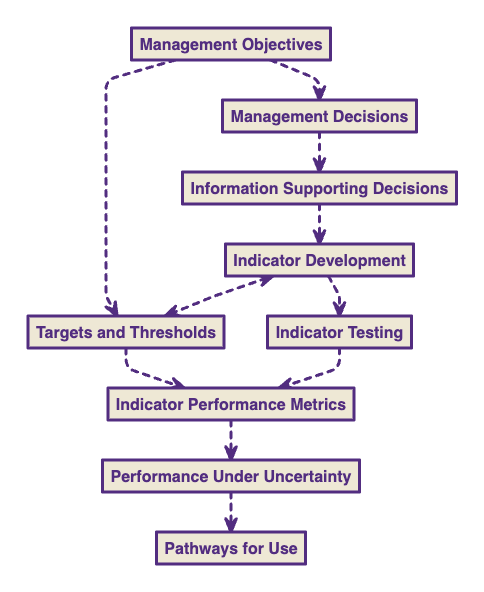
\includegraphics[width=1\linewidth]{MiniWK_Overview_files/figure-latex/projectoutline-1}

\begin{ltbluebox}
\emph{This workshop addresses project goals:}\\
* Review and assess existing indicators and evaluate their utility to
support management objectives\\
* Identify and develop priority ecosystem and habitat indicators,
including associated targets and thresholds as appropriate, and identify
specific pathways for incorporation into Council management processes

\end{ltbluebox}

\end{col}

\end{cols}

\end{document}
